\chapter{Model Architecture and Experiments}
\phantomsection
\label{ch:experiments}


\vspace{-1cm}
\setlength{\parindent}{0pt}
\vspace{0.3cm}

\section{End-to-End Khmer OCR Network system}
\label{sec:end_to_end_khmer_ocr_sysetm}

{\englishfont\fontsize{13.5pt}{17pt}\selectfont

We propose an end-to-end Khmer OCR pipeline that combines the CRAFT model 
for text detection with the TrOCR model architecture developed by Microsoft 
for text recognition. We have customized and adapted the system to support 
both Khmer and English languages. The pipeline takes an input image, applies 
the CRAFT model to detect and crop individual text-line regions, and then 
feeds each text-line image into the TrOCR model.
The TrOCR model operates in an auto-regressive manner, decoding one character 
at a time until it reaches the end-of-sequence token. This approach allows the 
system to handle variable-length input text-lines without any predefined limit, 
as long as the input fits within the model’s maximum token capacity.
This is a high-level description of the system architecture. Importantly, 
our pipeline operates without any preprocessing steps like binarization, 
noise removal, or skew adjustment. It processes raw input images directly, 
handling both detection and recognition seamlessly within a unified end-to-end 
framework.

\section{Experimental Environment and Tools}
\label{sec:environment}

All experiments were conducted on a Linux CLI system with the following hardware
and software specifications listed below:

\begin{table}[H]
    \centering
    \caption{Experimental Setup and Environment Configuration}
    \renewcommand{\arraystretch}{1.4}
    \resizebox{\textwidth}{!}{%
    \begin{tabular}{|p{4.5cm}|p{5.7cm}|p{6.5cm}|}
    \hline
    \textbf{Component} & \textbf{Specification} & \textbf{Purpose} \\[0.2cm]
    \hline
    \multicolumn{3}{|c|}{\textbf{Hardware Configuration}} \\[0.2cm]
    \hline
    Operating System & Ubuntu 20.04 LTS & Stable training large model \\[0.2cm]
    \hline
    GPU Units & 3x NVIDIA RTX 4090 & Parallel computing \\[0.2cm]
    \hline
    VRAM & 24 GB per GPU (72 GB total) & Large model training and inference \\[0.2cm]
    \hline
    System Memory & 256 GB RAM & Great for loading \& processing \\[0.2cm]
    \hline
    \multicolumn{3}{|c|}{\textbf{Software Framework}} \\[0.2cm]
    \hline
    DL Framework & PyTorch & implementation \& training \\[0.2cm]
    \hline
    Model Library & Hugging Face Transformers & Pre-trained architecture access \\[0.2cm]
    \hline
    GPU Acceleration & CUDA & Great for training across GPUs \\[0.2cm]
    \hline
    \multicolumn{3}{|c|}{\textbf{Experiment Management}} \\[0.2cm]
    \hline
    Tracking System & MLflow & Real-time metric logging \\[0.2cm]
    \hline
    Monitored Metrics & CER, Train/Valid Loss & evaluation \& comparison \\[0.2cm]
    \hline
    \end{tabular}%
    }
    \label{tab:experimental_setup}
\end{table}

\section{CRAFT for Text Detection}
\label{sec:craft-complete}

This section presents a comprehensive overview of the CRAFT 
(Character Region Awareness for Text Detection) model implementation, 
covering its architecture, configuration, training methodology, dataset 
preparation, and evaluation metrics.

\subsection{CRAFT Model Architecture}
\label{subsec:craft-architecture}

For the text detection stage, we adopted the Character Region Awareness for Text 
Detection (CRAFT) model, which is a fully convolutional network architecture 
based on VGG-16 with batch normalization is adopted as this architecture's backbone.
The model has skip connections in the decoding part, which is similar to U-net in
that aggregates low-level features. The final output is producing two channels as 
score maps:
\begin{itemize}
\item A \textbf{region score map}, indicating the likelihood of each pixel belonging 
to a character region.
\item An \textbf{affinity score map}, capturing the spatial relationships between 
adjacent characters to form text lines.
\end{itemize}

Unlike traditional text detectors that rely on bounding-box regression, 
CRAFT performs pixel-level predictions to detect the centers of individual 
characters and the affinities between them, allowing it to handle curved, 
rotated, or irregular text effectively. However, in our work, we focus on 
text-line-level detection rather than character-level because Khmer is a 
complex writing system. Many characters are visually dependent, invisible, 
or cannot appear independently, making character-level detection unreliable 
for curved or rotated Khmer text. Since curved text detection relies on accurate 
per-character localization and grouping, CRAFT's character-centric design does 
not perform well on curved Khmer scripts.



\begin{figure}[H]
    \centering
    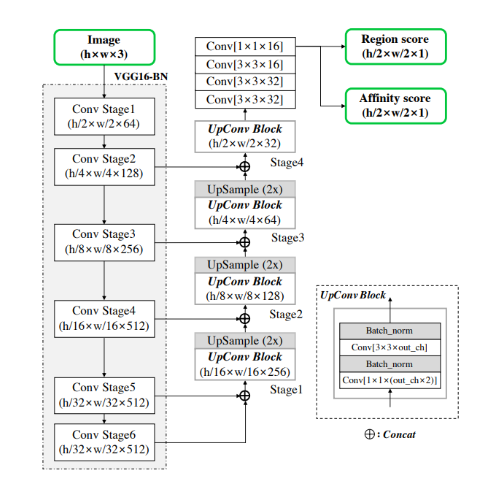
\includegraphics[width=\textwidth]{figures/craft_layer_network.png}
    \caption{Schematic illustration of our CRAFT network architecture.
    \citep{baek2019craft}}
    \label{fig:craft-model}
\end{figure}


\subsection{CRAFT Network Architecture}
\label{subsec:craft-architecture-network}

The Character Region Awareness for Text Detection (CRAFT) model adopts a fully convolutional architecture based on the VGG-16 backbone with batch normalization. It is designed to predict two output maps: the region score map and the affinity score map, representing the center probability of each character and the space between adjacent characters, respectively.

\subsubsection*{Backbone Network: VGG-16}

The first part of the model utilizes VGG-16 \cite{Simonyan} 
as the feature extractor. Let the input image be denoted by 
$I \in \mathbb{R}^{H \times W \times 3}$. The VGG-16 backbone extracts 
hierarchical feature maps:

\[
\begin{aligned}
F_1 &= \text{Conv}_{1\text{-}2}(I) \quad &\text{(features after conv1)} \\
F_2 &= \text{Conv}_{2\text{-}2}(F_1) \quad &\text{(features after conv2)} \\
F_3 &= \text{Conv}_{3\text{-}3}(F_2) \quad &\text{(features after conv3)} \\
F_4 &= \text{Conv}_{4\text{-}3}(F_3) \quad &\text{(features after conv4)} \\
F_5 &= \text{Conv}_{5\text{-}3}(F_4) \quad &\text{(features after conv5)} \\
\end{aligned}
\]

\subsubsection*{Decoder: U-Net-style Feature Fusion}

The decoder employs a U-Net-like architecture \cite{Ronneberger} with skip 
connections to aggregate semantic and spatial information. Starting from $F_5$, 
the features are upsampled and concatenated with features from earlier layers:

\[
\begin{aligned}
F_{54} &= \text{Concat}(\text{Upsample}(F_5), F_4) \\
F_{543} &= \text{Concat}(\text{Upsample}(F_{54}), F_3) \\
F_{5432} &= \text{Concat}(\text{Upsample}(F_{543}), F_2) \\
F_{54321} &= \text{Concat}(\text{Upsample}(F_{5432}), F_1) \\
\end{aligned}
\]

Each fusion step is followed by one or more $3 \times 3$ convolutional layers with ReLU activations. The final decoding stage uses a series of convolution layers:

\[
\text{Conv}_{3\times3\times32} \rightarrow \text{Conv}_{3\times3\times32} \rightarrow \text{Conv}_{3\times3\times16} \rightarrow \text{Conv}_{1\times1\times16}
\]

\subsubsection*{Output Heads}

The final fused features are projected into two separate output maps using $1 \times 1$ convolutions:

\[
\begin{aligned}
S_r &= \sigma(\text{Conv}_{1\times1}^{1}(F_{out})) \quad &\text{(region score map)} \\
S_a &= \sigma(\text{Conv}_{1\times1}^{1}(F_{out})) \quad &\text{(affinity score map)} \\
\end{aligned}
\]

Here, $\sigma$ denotes the sigmoid activation function. 
The region score $S_r$ represents the likelihood that a pixel is at the center 
of a character, while the affinity score $S_a$ represents the connection strength 
between adjacent characters \citet{baek2019craft}.

\subsubsection*{Output Resolution}

The output maps $S_r$ and $S_a$ are of size $H' \times W'$, 
typically at $\frac{1}{2}$ resolution of the input image due to strided 
convolutions and pooling operations in the VGG-16 backbone.










\begin{figure}[H]
    \centering
    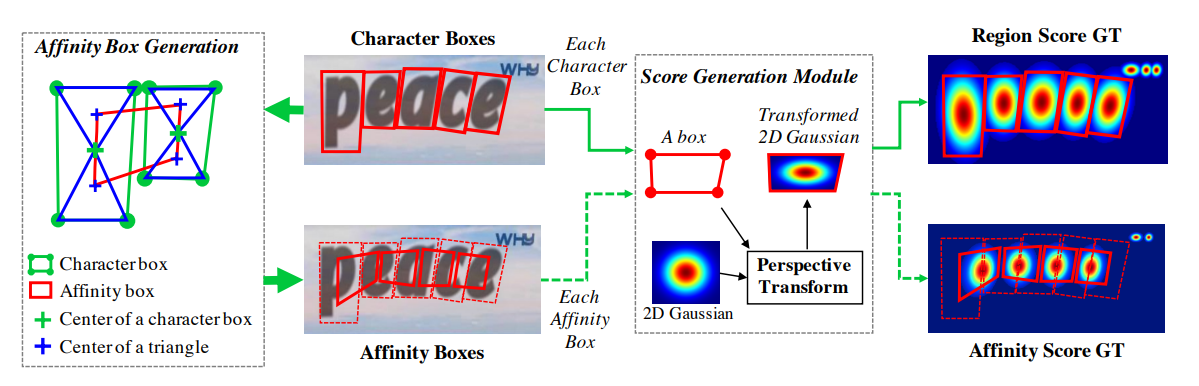
\includegraphics[width=\textwidth]{figures/craft_model_architecture.png}
    \caption{Illustration of ground truth generation procedure in our framework. 
    We generate ground truth labels from a synthetic image that has character level annotations.
    \citep{baek2019craft}}
    \label{fig:craft-model-architecture-detailed}
\end{figure}

The model has 20,770,466 trainable parameters. We used the official 
implementation of CRAFT with some modifications to better support Khmer text,
including the use of a custom dataset and a modified training procedure such as
skip the character labels during training.


\subsection{CRAFT Training Configuration}
\label{subsec:craft-training-config}

The CRAFT model was fine-tuned on a custom Khmer text dataset using fully supervised learning, 
leveraging the strengths of annotated real-world images. The key configuration parameters 
for training the CRAFT model are summarized in Table~\ref{tab:craft-training-config}.

\begin{table}[H]
    \renewcommand{\arraystretch}{1.3} % Adjusts row height
    \centering
    \begin{tabular}{|p{0.4\linewidth}|p{0.55\linewidth}|}
    \hline
    \textbf{Parameter} & \textbf{Value} \\
    \hline
    Backbone architecture & VGG-16 \\
    Pretrained weights & \texttt{CRAFT.pth} \\
    Batch size & 8 \\
    Training iterations & 0 to 10,000 \\
    Evaluation interval & Every 500 iterations \\
    Learning rate & 0.0001 \\
    Optimizer & Adam \\
    Input image size & 768px (height, aspect ratio preserved) \\
    \hline
    \end{tabular}
    \caption{Key configuration parameters for training the CRAFT model on a custom Khmer dataset using strong supervision.}
    \label{tab:craft-training-config}
\end{table}


\subsection{Dataset for Text Detection}
\label{subsec:craft-dataset}

{\englishfont The dataset preparation for CRAFT model training involved a comprehensive manual 
annotation process where text-line regions were annotated one by one with precise 
bounding boxes. This highly approach ensured high-quality ground truth data 
that accurately captured the complex structure of Khmer script, including its 
unique diacritics, ligatures, and stacked character arrangements.
To accelerate the annotation process while maintaining accuracy, we integrated 
commercial APIs, specifically Google's text detection API, as an initial automated 
annotation step. However, since these commercial APIs are not perfect and often 
struggle with Khmer script complexity, each automatically generated bounding box 
required manual verification and correction. }


\begin{figure}[H]
    \centering
    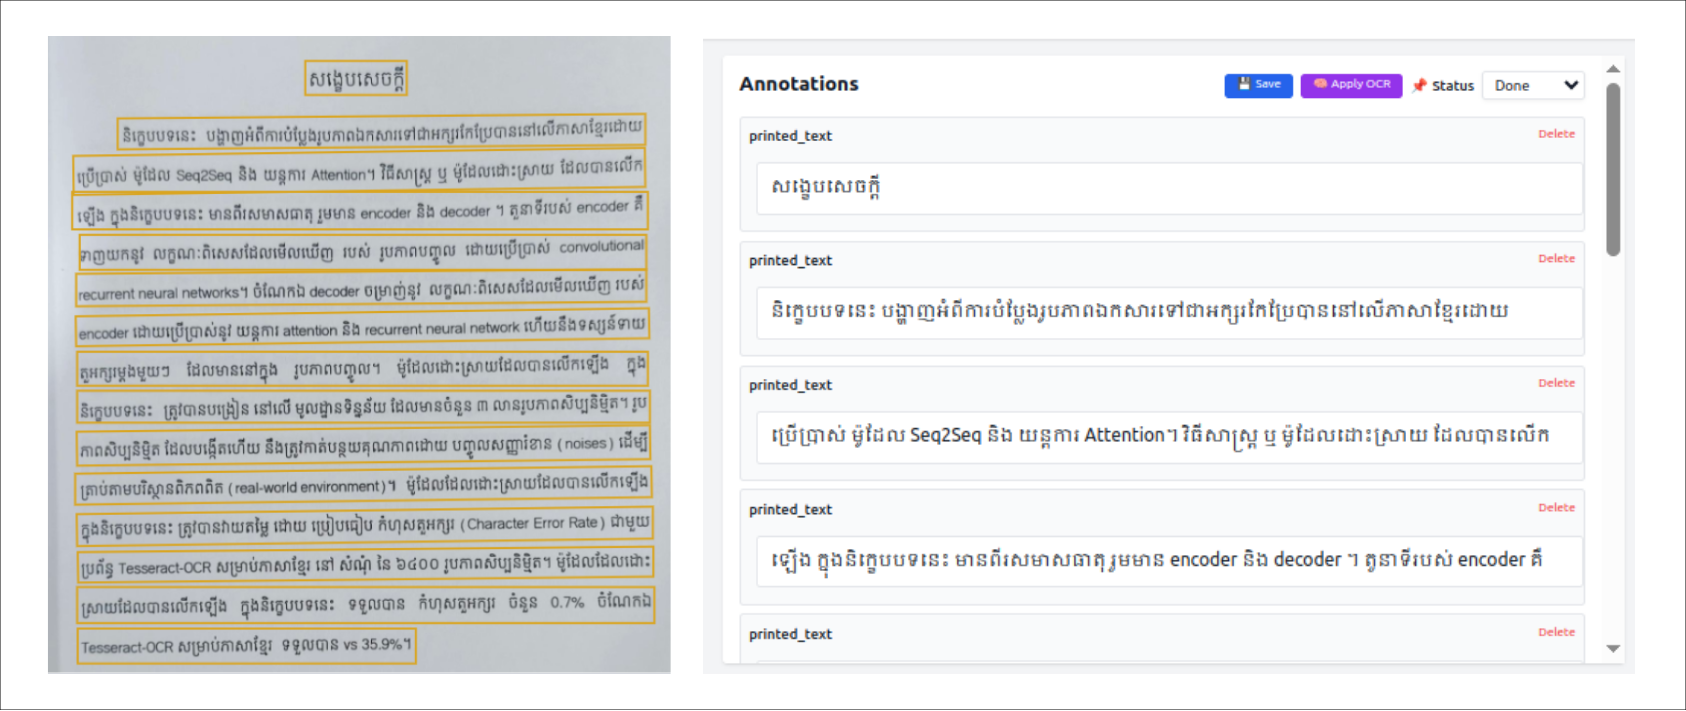
\includegraphics[width=\textwidth]{figures/craft_text_annotation.png}
    \caption{\englishfont The example of text detection dataset collection using commercial API}
    \label{fig:data_craft_collection}
\end{figure}


{\englishfont This hybrid approach significantly 
reduced annotation time while ensuring the final dataset quality met our standards.
The entire data collection and annotation process was facilitated by a custom-built 
annotation tool developed specifically for this project. This tool was designed with 
easy integration capabilities for commercial APIs, allowing seamless incorporation of 
automated suggestions while providing intuitive interfaces for manual correction 
and refinement. The tool's flexible architecture enabled rapid switching between 
different API providers and manual annotation modes, optimizing the overall annotation 
workflow.
Throughout the training process, a variety of data augmentation techniques were 
employed to enhance the model's robustness against font diversity, image noise, 
and other real-world distortions.

These transformations enriched the training set with diverse visual variations, 
which helped the model generalize more effectively to unseen data. The final 
manually annotated dataset comprised 7000 high-quality bounding boxes that captured 
the intricate structure of the Khmer script, ensuring robust training data for the 
CRAFT model fine-tuning process. }



\subsection{CRAFT Training Experiment}
\label{subsec:craft-training-results}

{\englishfont
The CRAFT model was evaluated during training using precision, recall, and Intersection over
Union (IoU) metrics. The text detection model demonstrated excellent performance in detecting text 
regions with high accuracy as you can see in the Figure~\ref{fig:iou-recall-craft}.
}
 
\begin{figure}[H]
    \centering
    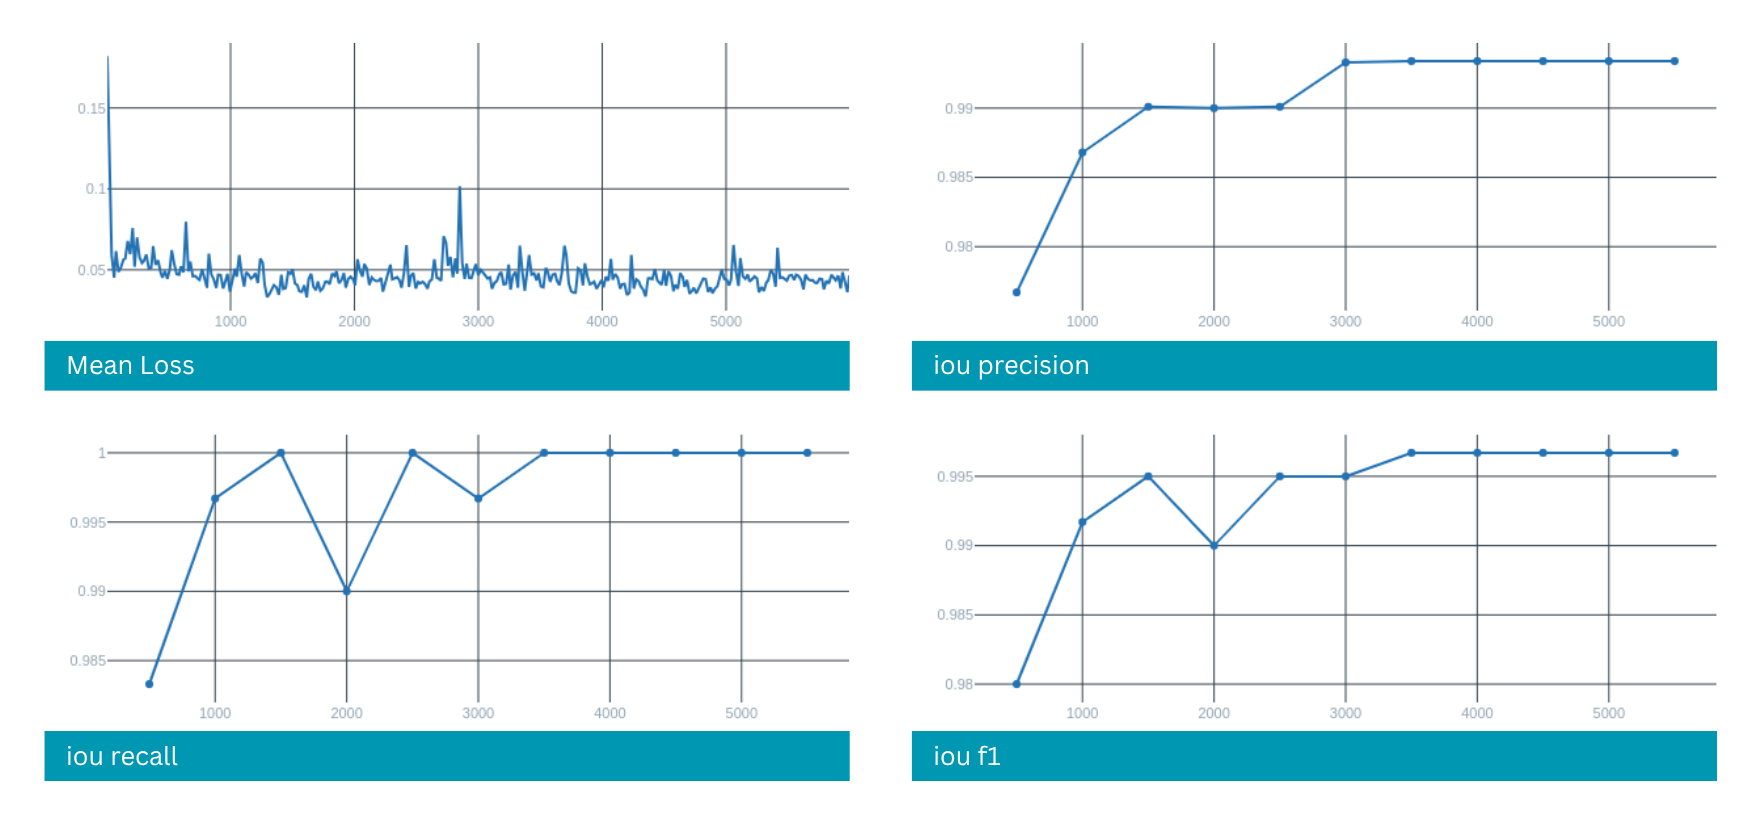
\includegraphics[width=\textwidth]{figures/craft_traning_process_5000.png}
    \caption{Illustration of the recall, precision, and the intersection over union 
    (IOU) performance of the CRAFT model with 5000 steps.}
    \label{fig:iou-recall-craft}
\end{figure}



\section{TrOCR for Text Recognition}
\label{sec:trocr-complete}

This section provides a comprehensive examination of the TrOCR (Transformer-based Optical Character Recognition) model implementation, including its architecture, customization for Khmer script, training methodology, and evaluation results.

\subsection{TrOCR Model Architecture}   
\label{subsec:trocr-architecture-architecture}

For the text recognition component of the pipeline, we used the \textbf{TrOCR} model, a transformer-based OCR system proposed by Microsoft Research. TrOCR stands for \textit{Transformer-based Optical Character Recognition}, and it integrates a vision encoder with a language decoder in a unified encoder-decoder (Seq2Seq) architecture, following the structure of the Vision Transformer (ViT) and pre-trained language models like BART.

The TrOCR model takes the cropped text-line image detected by CRAFT and processes it through a \textbf{ViT-based encoder}, which extracts rich visual features. These features are then passed to the \textbf{transformer decoder}, which generates the text sequence token-by-token, using cross-attention to focus on relevant image features while decoding. This allows the model to handle complex scripts like Khmer with better accuracy and context-awareness.

\begin{figure}[H]
    \centering
    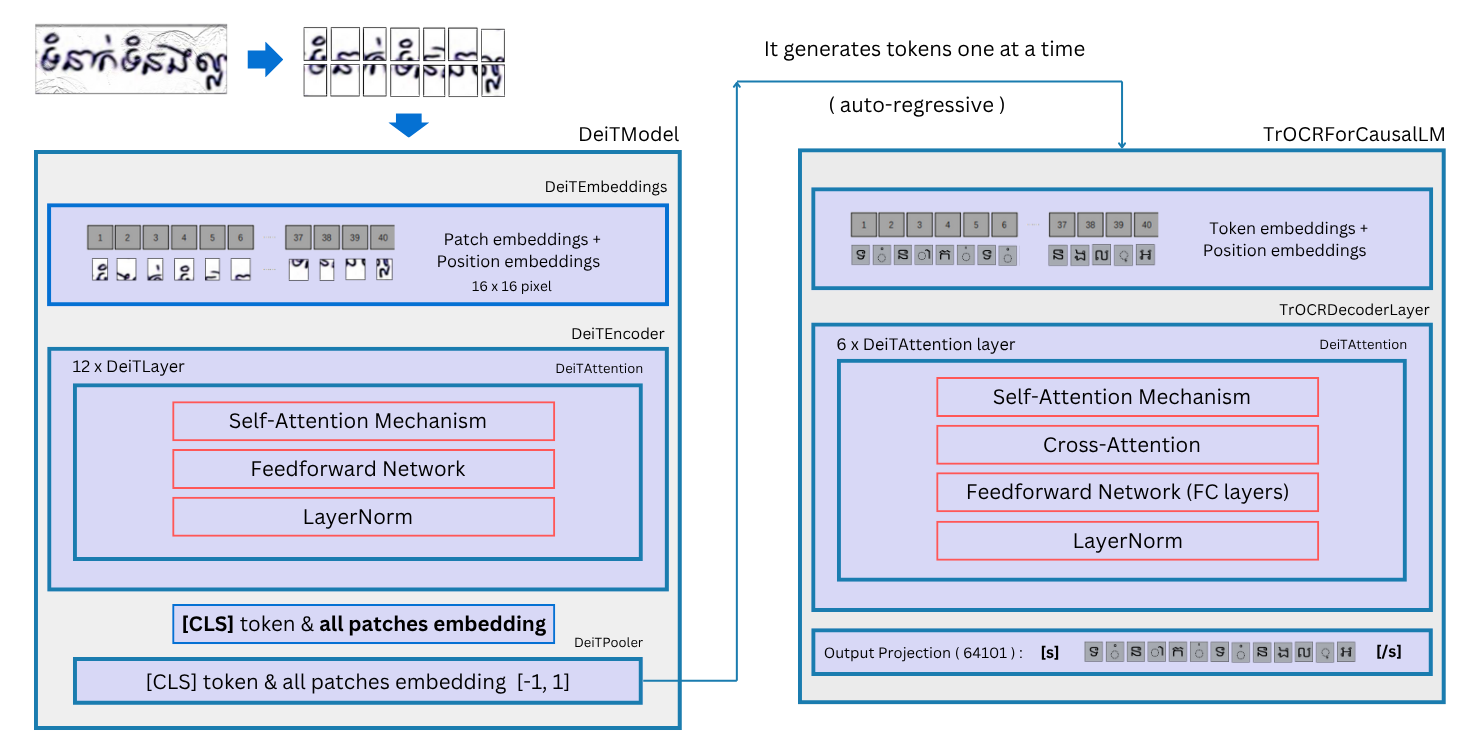
\includegraphics[width=\textwidth]{figures/trocr_model.png}
    \caption{Illustration of the TrOCR model architecture used for text recognition.}
    \label{fig:trocr-model}
\end{figure}


\subsection{Architecture Overview}
\label{subsec:trocr-architecture-overview}  

The TrOCR architecture consists of two main components~\cite{li2021trocr}:

\begin{itemize}
    \item \textbf{Vision Encoder:} A pre-trained Vision Transformer (ViT)~\cite{dosovitskiy2020image}, which
     extracts a sequence of visual features from input images.
    \item \textbf{Text Decoder:} A GPT-2-style autoregressive transformer that 
    generates character sequences from the visual features \cite{li2021trocr}.
\end{itemize}

Let the input image be denoted as $I \in \mathbb{R}^{H \times W \times 3}$.

\subsubsection*{Encoder: Vision Transformer}

The image $I$ is split into a sequence of $N$ patches, each of size $P \times P$. 
These patches are linearly projected into embeddings and processed through a Transformer encoder:

\[
x_0 = [\text{CLS}; x^1; x^2; \dots; x^N] + E_{pos}
\]

\[
Z = \text{TransformerEncoder}(x_0)
\]

where $x^i$ is the $i$-th patch embedding, $E_{pos}$ is the 
positional encoding, and $Z \in \mathbb{R}^{N \times D}$ is the final visual 
feature representation of the image.

\subsubsection*{Decoder: Autoregressive Transformer}

The decoder takes the encoder's output $Z$ and generates a 
character sequence $y = (y_1, y_2, \dots, y_T)$:

\[
P(y_t | y_{<t}, Z) = \text{softmax}(W_o h_t)
\]

\[
h_t = \text{DecoderBlock}(y_{<t}, Z)
\]

where $W_o$ is the output projection matrix and $h_t$ is the hidden state at time step $t$.




\subsection{Custom TrOCR Processor for Interpretability on Khmer}
\label{subsec:trocr-customization}

To make the TrOCR model understand Khmer tokens, we customized the processor without modifying the original model architecture. We developed a CustomKhmerTokenizer based on a predefined list of unique Khmer and English characters, including special tokens such as \textit{<s>}, \textit{</s>}, and \textit{<pad>}, to handle the encoding of text into token IDs and the decoding of token IDs back into readable text.

This tokenizer was then wrapped inside a custom processor that mimics the behavior of Hugging Face's TrOCRProcessor, allowing seamless integration with TrOCR's image processing pipeline. By doing so, we enabled the model to work with Khmer script during both training and inference, while preserving the original TrOCR model's structure and leveraging its pretrained capabilities.

\begin{figure}[H]
    \centering
    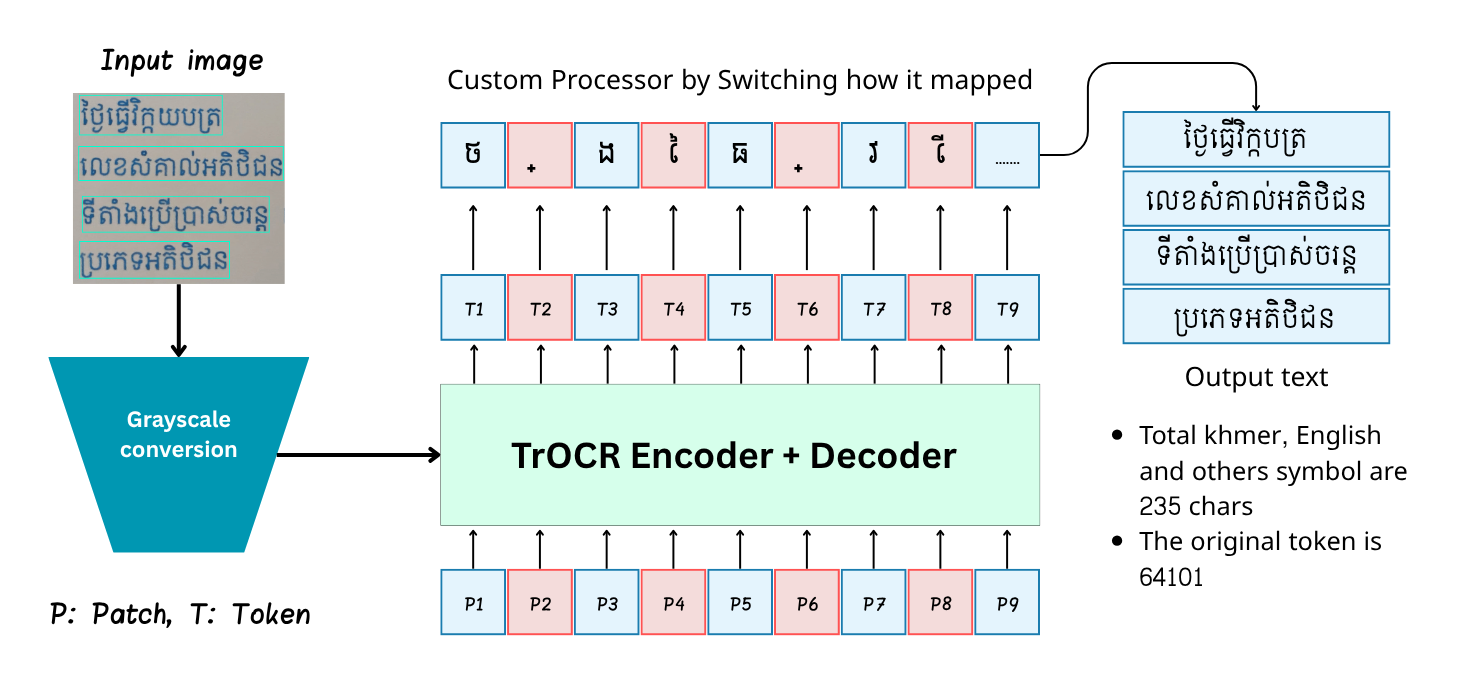
\includegraphics[width=\textwidth]{figures/Customize_processor.png}
    \caption{Architecture of the customized TrOCR pipeline. 
    The original TrOCR model is extended with a custom processor, 
    which is tailored for Khmer character decoding.}
    \label{fig:trocr-custom-processor}
\end{figure}

\subsection{Training TrOCR Workflow}
\label{subsec:trocr-training}

For the TrOCR model, we selected the base model because we were working with a multilingual dataset and wanted the model to have sufficient parameter capacity for this task. The training dataset consisted of 7.4 million synthetic images generated using our text-to-image pipeline.

\begin{figure}[H]
    \centering
    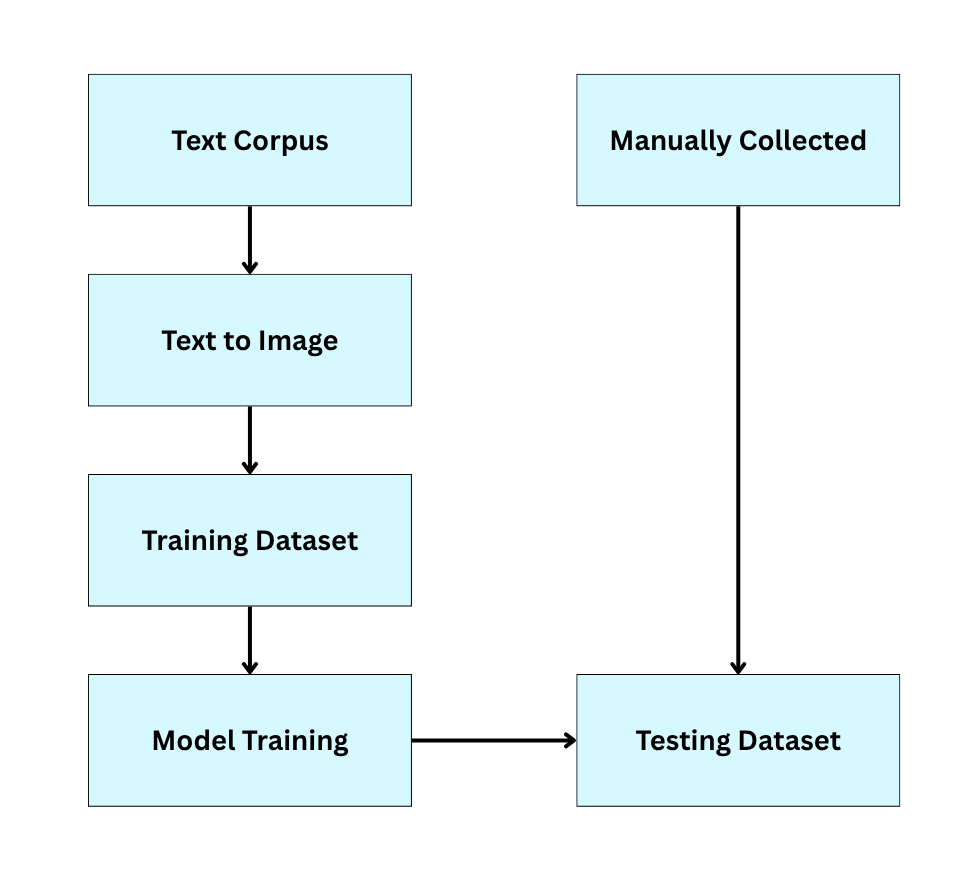
\includegraphics[width=\textwidth]{figures/trocr_model_overflow_training.png}
    \caption{Overview of the TrOCR training process. Text-generated 
    images form the training set, while real-world samples are 
    manually collected for testing and evaluation.}
    \label{fig:trocr-training-pipeline}
\end{figure}

The choice of batch size 1024 was crucial for model generalization. Initial experiments with smaller batch sizes (8, 16, 32, 128, 256) resulted in severe overfitting, as demonstrated in Figure~\ref{fig:trocr-overfitting}.

\subsection{TrOCR Training Results and Performance}
\label{subsec:trocr-training-results}

After experimenting with different hyperparameters, we found the optimal configuration:
\begin{itemize}
\item \textbf{Batch size}: 1024
\item \textbf{Learning rate}: 0.00001
\item \textbf{Epochs}: 3
\item \textbf{Dataset size}: 7.4 million images
\end{itemize}


\begin{figure}[H]
    \centering
    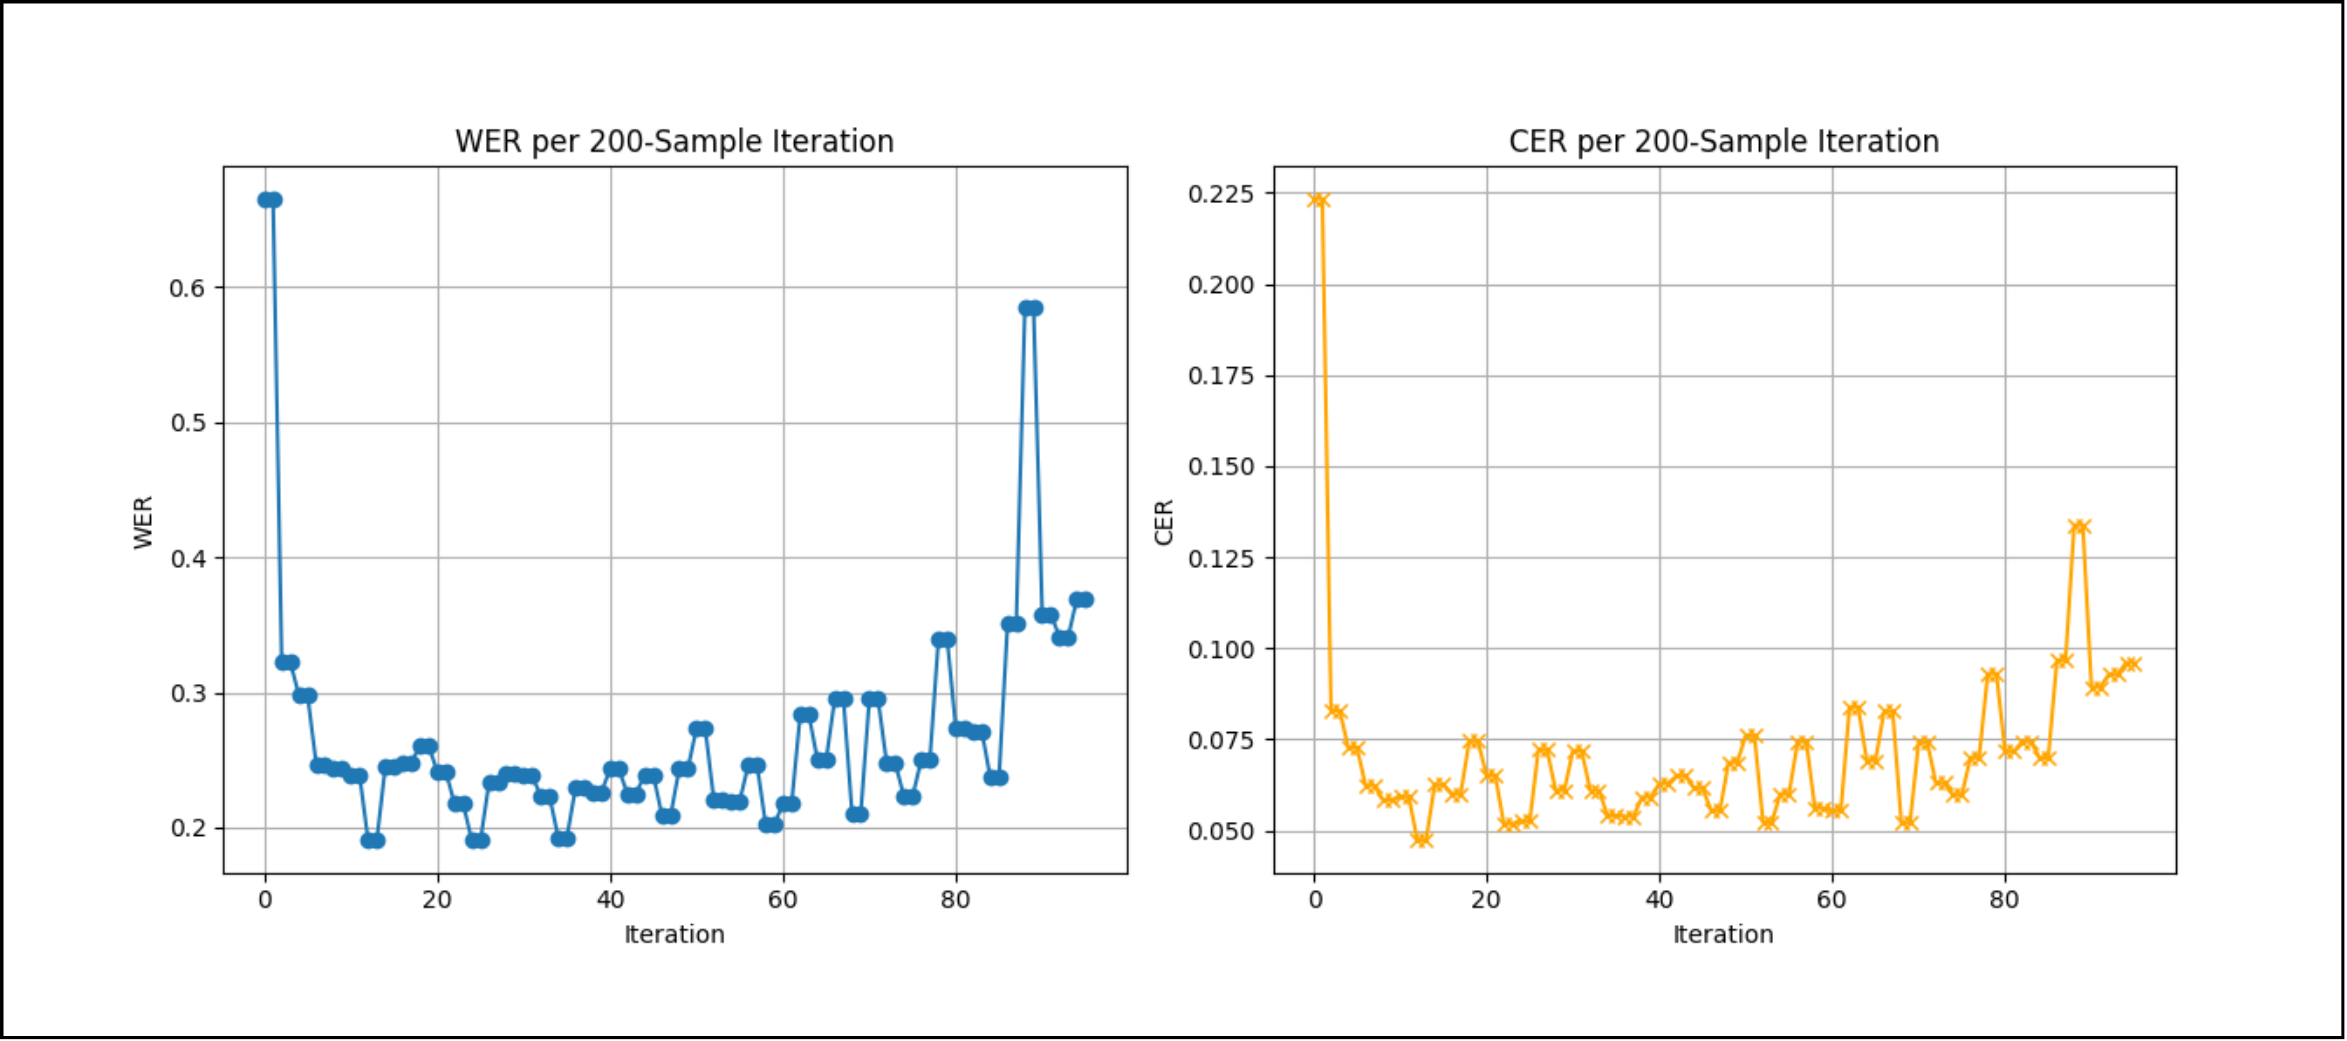
\includegraphics[width=\textwidth]{figures/trocr_overfitting_v1.png}
    \caption{Training and validation loss curves for TrOCR model with batch size 8, 
    clearly showing overfitting behavior where training loss decreases while validation loss increases.}
    \label{fig:trocr-overfitting}
\end{figure}

The graph above illustrates a clear case of overfitting when using a batch size of 8. The training loss continues to decrease while the validation loss starts to increase, indicating that the model learns very specific patterns from the training data rather than generalizing well to unseen data.

\begin{figure}[H]
    \centering
    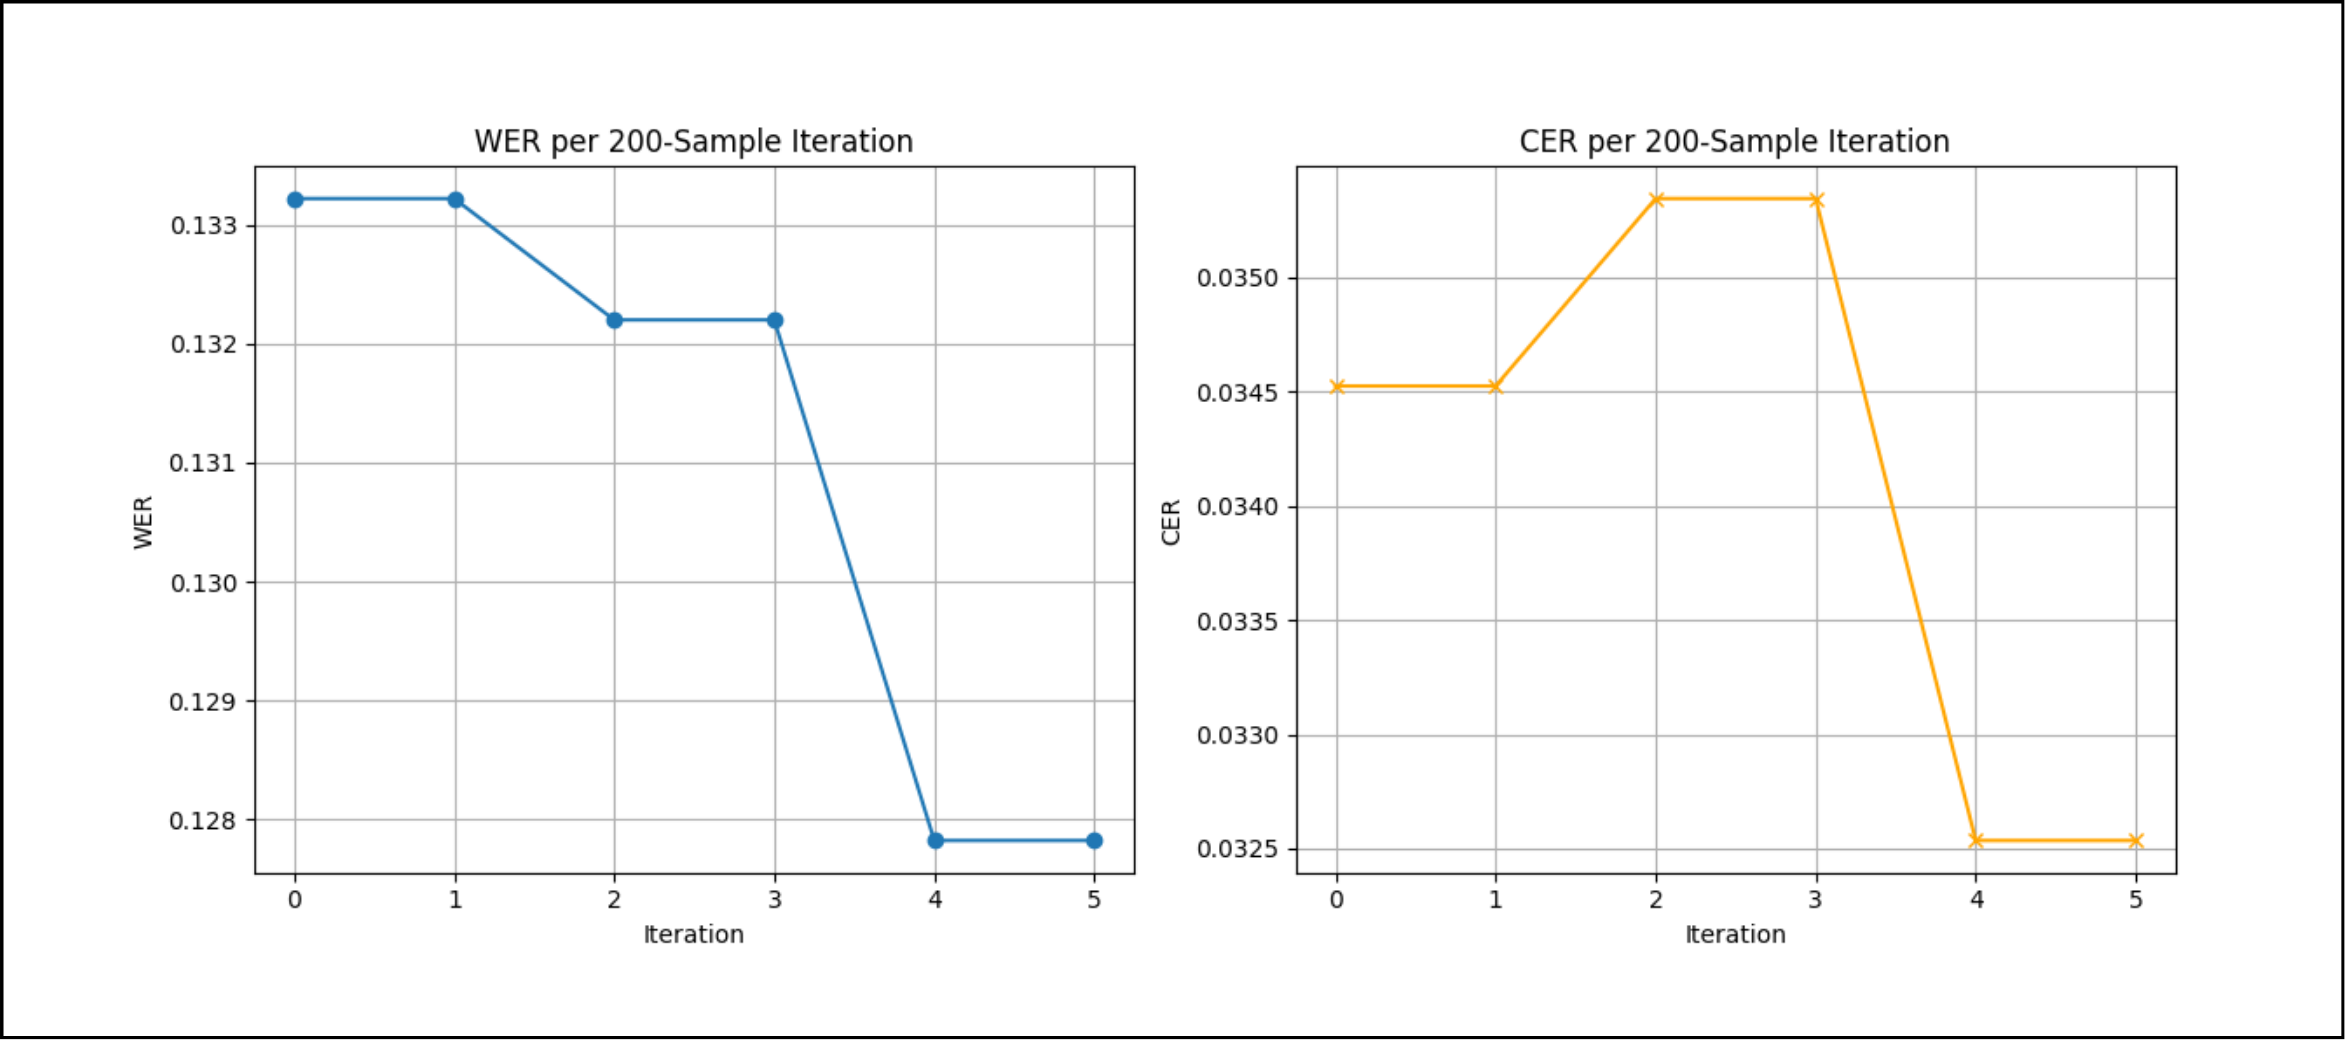
\includegraphics[width=\textwidth]{figures/trocr_fine_tuning.png}
    \caption{Training and validation metrics for TrOCR model with batch size 1024, 
    showing Character Error Rate (CER) and Word Error Rate (WER) over training steps. 
    The model demonstrates excellent performance from early training steps, with CER quickly 
    reaching around 0.03 and WER staying below 0.12.}
    \label{fig:trocr-fine-tuning}
\end{figure}

With the optimized batch size of 1024, the model showed remarkable performance from early stages of training, with CER quickly stabilizing around 0.03 and WER maintaining values below 0.12. This rapid convergence can be attributed to the utilization of pretrained weights and the larger batch size enabling better generalization.


\section{End-to-End OCR Pipeline}
\label{sec:end-to-end-pipeline}

This section describes the integration of CRAFT and TrOCR models into a unified end-to-end OCR system capable of processing multilingual documents containing both Khmer and English text.

\subsection{Pipeline Architecture}
\label{subsec:pipeline-architecture}

The overall workflow is presented in Figure~\ref{fig:trocr-inference-full-pipeline}. The pipeline begins with input images containing English and Khmer text, or mixed-language content. The preprocessing step converts images to grayscale to streamline downstream processing and improve model prediction accuracy.

\begin{figure}[H]
    \centering
    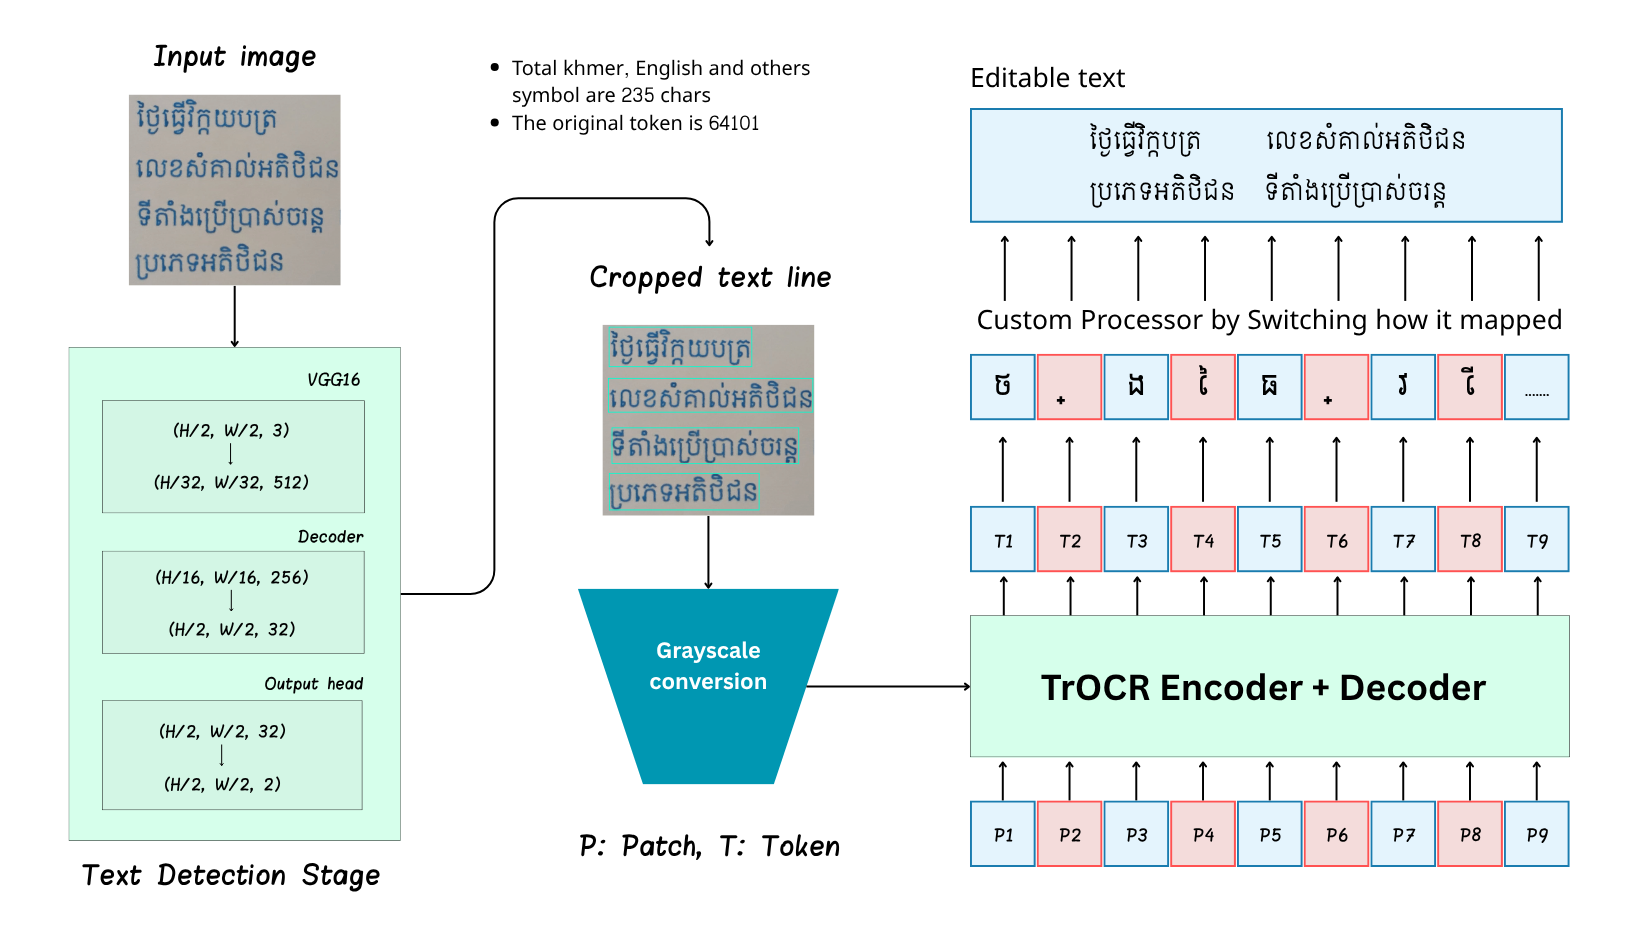
\includegraphics[width=\textwidth]{figures/khmerOCR_inference_full_pipeline.png}
    \caption{End-to-end OCR inference pipeline for converting text images into digital text.}
    \label{fig:trocr-inference-full-pipeline}
\end{figure}

\subsection{Pipeline Processing Steps}
\label{subsec:pipeline-steps}

The complete pipeline operates through the following sequential steps:

\begin{enumerate}
\item \textbf{Image Preprocessing}: Input images are converted to grayscale and normalized to ensure consistent processing across different image types and qualities.

\item \textbf{Text Detection}: The CRAFT model detects text regions in the image on a text-line basis, generating bounding boxes for each detected text segment.

\item \textbf{Post-processing and Reordering}: Detected text-lines undergo post-processing to ensure correct reading order, accounting for document layout and text flow patterns.

\item \textbf{Text-line Cropping}: Individual text-line regions are extracted from the original image based on CRAFT detection results.

\item \textbf{Text Recognition}: Each cropped text-line image is processed by the TrOCR model to generate the corresponding digital text output.

\item \textbf{Output Assembly}: Recognized text from all text-lines is assembled in the correct order to produce the final digital document.
\end{enumerate}

\subsection{Pipeline Integration Benefits}
\label{subsec:pipeline-benefits}

The integration of CRAFT and TrOCR provides several advantages:

\begin{itemize}
\item \textbf{Character-level Detection}: CRAFT's character-aware detection is particularly effective for complex scripts like Khmer with stacked characters and diacritics.

\item \textbf{Transformer-based Recognition}: TrOCR's attention mechanism allows for better context understanding and improved accuracy on both Khmer and English text.

\item \textbf{Multilingual Support}: The pipeline seamlessly handles documents containing both Khmer and English text without requiring language-specific preprocessing.

\item \textbf{End-to-end Processing}: The unified pipeline eliminates the need for manual intervention between detection and recognition stages.
\end{itemize}

This comprehensive approach ensures robust performance across diverse document types and text conditions, making it suitable for real-world OCR applications in multilingual environments.

}